\documentclass[fleqn,12pt]{article}

\usepackage[margin=15mm]{geometry}
\usepackage[utf8]{inputenc}
\usepackage[bulgarian]{babel}
\usepackage[unicode]{hyperref}
\usepackage{amsthm}
\usepackage{amssymb}
\usepackage{mathtools}
\usepackage[unicode]{hyperref}
\usepackage{enumitem, hyperref}
\usepackage{indentfirst}
\usepackage{graphics}

\renewcommand{\arraystretch}{1.3}   

\title{Navier-Stokes 2D - елементи}

\begin{document}
    
\maketitle

\tableofcontents
\pagebreak

\section{Триъгълни}

\subsection{4P1/P1}
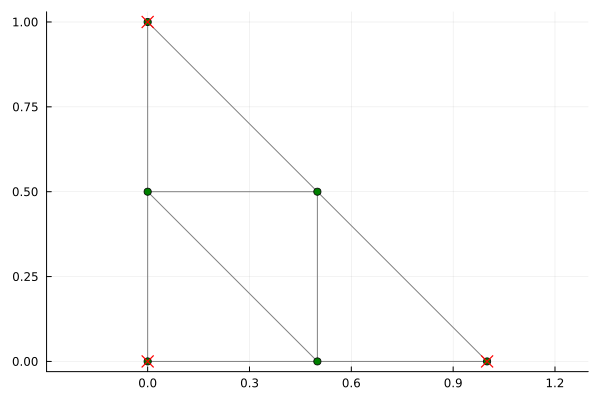
\includegraphics[width=140mm]{img/4p1p1.png}

Триъгълника се разцепва на четири, за да се елиминират осцилации в налягането ("spurious pressure modes").
Има и алтернативно разцепване - свързване на върховете с медицентъра.

\begin{verbatim}
https://sci-hub.se/https://doi.org/10.1146/annurev.fl.24.010192.001123
\end{verbatim}
\begin{itemize}
    \item Indeed a finite element method for thc Stokes problem
    introduced in Bercovier \& Pironneau (1979) was (implicitly) based on this
    idea. In the above reference one proves the convergence of a finite element
    approximation of the Stokes problem (4.1)-(4.3) (with 0: = 0 and r 0 = r),
    where one uses a continuous piecewise linear pressure on a triangulation
    :Yh/2' twice finer than :T,,; this finite element approximation will be described
    in the following Section 4.3.2
\end{itemize}

\begin{verbatim}
Implementation of Finite Element Methods for Navier-Stokes Equations
\end{verbatim}

\subsection{P1 + мехурче / P1 (MINI)}
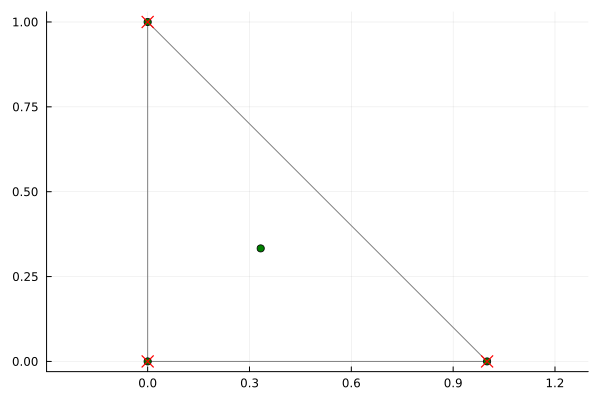
\includegraphics[width=140mm]{img/mini.png}
\begin{verbatim}
Larson, Bengzon: The finite element method (ISBN 3642332862) [стр. 301] 
\end{verbatim}
\begin{itemize}
    \item MINI element (P1 + bubble / P1)
    \item "However, it is also known for giving a poor approximation of the pressure"
\end{itemize}


\subsection{P2/P1 (Taylor-Hood)}
\begin{verbatim}
Larson, Bengzon: The finite element method (ISBN 3642332862) [стр. 301] 
\end{verbatim}
\begin{verbatim}
Implementation of Finite Element Methods for Navier-Stokes Equations
\end{verbatim}

\subsection{P2 + мехурче / P1*}
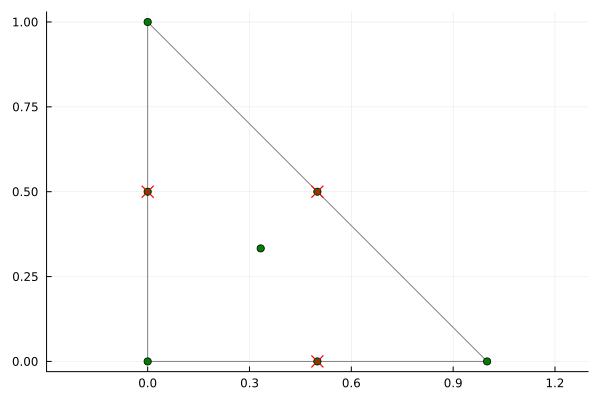
\includegraphics[width=140mm]{img/p2_bubble_p1.png}

Възлите за налягане могат да се разположат на произволно място.
Нарисувани са в центровете на страните, за да се покаже че налягането може да е прекъснато.
Добавката (мехурчето) е $q_7 xy(1-x-y)$, т.е. множител по произведението на линейните функции.
Оценките за грешките ($O(h^2)$) се постигат в специални норми (има subscript) - TODO.
В тях този елемент е оптимален.

\begin{verbatim}
Implementation of Finite Element Methods for Navier-Stokes Equations
\end{verbatim}
\begin{itemize}
\item $u_h$: "P2 + bubble" Triangle (or Modified P2); $p_h$: Discontinuous P1
\item bubble is third degree poly (composed of barycentric coords) with a single tuning parameter
\item $O(h^2)$ velocity and pressure accuracy
\item the nodes for the pressure can be chosen anywhere on the triangle
\end{itemize}

\subsection{6P1/P0 (Powell-Sabin)}
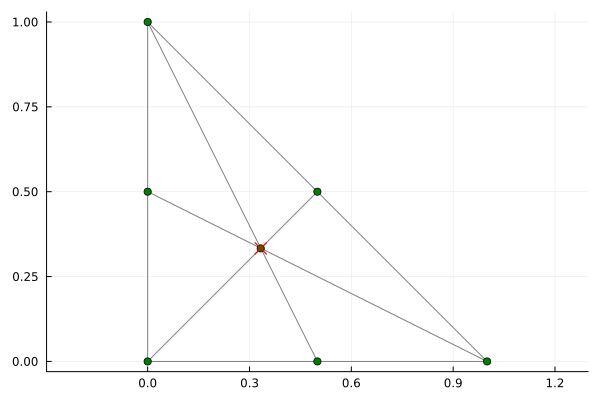
\includegraphics[width=140mm]{img/6p1p0.png}

Има divergence-free базис.

\begin{verbatim}
https://sci-hub.se/https://www.jstor.org/stable/43693550
\end{verbatim}
\begin{itemize}
    \item рисунката на стр. 463
\end{itemize}

\subsection{Неконформен P1/P0}
\begin{verbatim}
Larson, Bengzon: The finite element method (ISBN 3642332862) [стр. 301] 
\end{verbatim}
\begin{itemize}
    \item Crouzeix-Raviart (P1/P0 nonconforming)
    \item "This element has the desirable property of being able to yield a finite
       element solution that is exactly divergence free on each element"

\end{itemize}

\section{Правоъгълни}

\subsection{Q1/Q1 със стабилизация на налягането}

Стабилизацията на налягането е по метода на НМК (или поне много прилича).
Избора на силата на стабилизация е нетривиален.

\begin{verbatim}
https://web.archive.org/web/20170808232501id_/http://www.numerik.uni-hd.de/Oberwolfach-Seminar/CFD-Course.pdf
\end{verbatim}
    \begin{itemize}
        \item In order to get a stable discretization, it was proposed by Hughes et al. [49],
        to add certain least squares terms in the continuity equation
\end{itemize}
    

\subsection{Q2/Q1}
\begin{verbatim}
https://digitalcommons.pvamu.edu/cgi/viewcontent.cgi?article=1647&context=aam    
\end{verbatim}
\begin{itemize}
    \item Rectangular, 8 pts for velocity (quadratic interp), 4 pts for pressure (bilinear interp)
    \item Direct formulation, solved using Picard iteration
\end{itemize}

\subsection{Завъртян билинеен Q1/Q0}
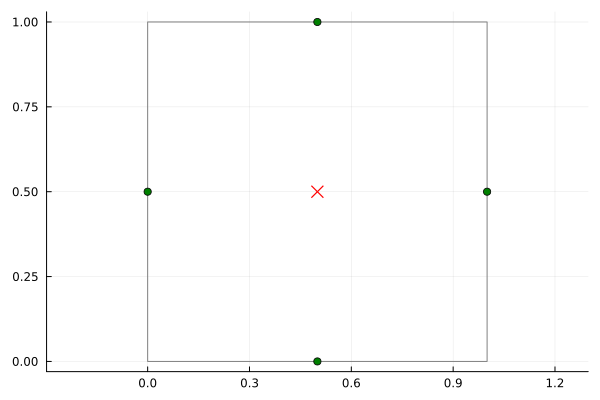
\includegraphics[width=140mm]{img/rotbl.png}

Има тънък момент с прехвърлянето към стандартни координати при нерегулиряни мрежи.
Трансформацията на координатите е от различен ред, което причинява проблеми.
Има заообикаляне.

\begin{verbatim}
https://web.archive.org/web/20170808232501id_/http://www.numerik.uni-hd.de/Oberwolfach-Seminar/CFD-Course.pdf
\end{verbatim}
\begin{itemize}
    \item It possesses a “divergence-free” nodal-basis, which allows the elimination of the pressure from the problem resulting in a positive definite algebraic
system for the velocity unknowns alone. The reduced algebraic system can be
solved by specially adapted multigrid methods; see Turek
\end{itemize}

\end{document}